\documentclass{beamer}

\usepackage[utf8]{inputenc}
%\usepackage{beamerthemesplit}
\usepackage{url}
\usepackage{tikz}
\usepackage{alltt}
\usepackage{listings}
\usepackage{marvosym}
\usepackage{color}
\usepackage[multidot]{grffile}
\usepackage{multirow}
\usepackage{array}
\usepackage{setspace}
\usepackage{hyperref}
\usepackage{verbatim}
\usepackage{fancyvrb}
%\hypersetup{colorlinks=true, linkcolor=blue,  anchorcolor=blue,  
%citecolor=blue, filecolor=blue, menucolor=blue, pagecolor=blue,  
%urlcolor=blue} 
\lstset{keywordstyle=\bfseries\color{brown},
        stringstyle=\ttfamily,
        commentstyle=\color{blue}\textit,
        showstringspaces=false}

\useoutertheme{}
\usetheme{Madrid}
\graphicspath{{pics/}{global/}
{pics/I/}{pics/A1/}{pics/A2/}{pics/A3/}{pics/A4/}{pics/A5/}{pics/A6/}{pics/A7/}
}

\logo{\includegraphics[height=1cm]{ProcessHorizontal}} 

\institute{Center for Computation and Technology\\Louisiana State University, Baton Rouge, LA}

\setbeamertemplate{navigation symbols}{} 

\title{CSC 7700: Scientific Computing}

% We want to use the infolines outer theme because it does not use a lot of
% space, but it also tries to print an institution and the slide
% numbers (which we might not want to show). Therefore, we here redefine the
% footline ourselfes - mostly a copy & paste from
% /usr/share/texmf/tex/latex/beamer/themes/outer/beamerouterthemeinfolines.sty
\defbeamertemplate*{footline}{infolines theme without institution and slide numbers}
{
  \leavevmode%
  \hbox{%
  \begin{beamercolorbox}[wd=.25\paperwidth,ht=2.25ex,dp=1ex,center]{author in head/foot}%
    \usebeamerfont{author in head/foot}\insertshortauthor
  \end{beamercolorbox}%
  \begin{beamercolorbox}[wd=.5\paperwidth,ht=2.25ex,dp=1ex,center]{title in head/foot}%
    \usebeamerfont{title in head/foot}\insertshorttitle
  \end{beamercolorbox}%
  \begin{beamercolorbox}[wd=.25\paperwidth,ht=2.25ex,dp=1ex,center]{date in head/foot}%
    \usebeamerfont{date in head/foot}\insertshortdate{}
  \end{beamercolorbox}}%
  \vskip0pt%
}

% Some useful commands
\newcommand{\abspic}[4]
 {\vspace{ #2\paperheight}\hspace{ #3\paperwidth}\includegraphics[height=#4\paperheight]{#1}\\
  \vspace{-#2\paperheight}\vspace{-#4\paperheight}\vspace{-0.0038\paperheight}}

\newcommand{\picw}[4]{{
 \usebackgroundtemplate{
 \color{black}\vrule width\paperwidth height\paperheight\hspace{-\paperwidth}\hspace{-0.01\paperwidth}
 \hspace{#4\paperwidth}\includegraphics[width=#3\paperwidth, height=\paperheight]{#1}}\logo{}
 \frame[plain]{\frametitle{#2}}
}}
\newcommand{\pic}[2]{\picw{#1}{#2}{}{0}}

\newcommand{\question}[1]{\frame{\frametitle{#1}
 \begin{centering}\Huge #1\\\end{centering}
}}



%\usecolortheme[RGB={200,200,200}]{structure}

\subtitle[Module A]{{\large Module A: Basic Skills}\\*[0.3em]Lecture 1: Survival skills for Unix environments}
\author[\mbox{\includegraphics[height=0.6em]{fl_300}\hspace{0.5em}Frank Löffler}]{Dr Frank Löffler}
\date{August 30 2013}

\begin{document}

\frame{\titlepage}

\section*{Outline}
\frame{\tableofcontents}

\section{Unix / Linux}
\frame{\frametitle{}\begin{centering}\LARGE\insertsectionhead\\\end{centering}}

\frame[containsverbatim]{ \frametitle{Unix History}
 \begin{itemize}
  \item Originally developed in 1969 by a group of AT\&T employees at Bell Labs
  \item Today's Unix systems split into various branches
  \item Adoption of Unix by commercial start-ups, most notably Solaris, HP-UX and AIX
  \item In contrast to: Unix-like operating systems such as Linux and BSD descendants
  \item Designed to be portable, multi-tasking and multi-user in a time-sharing configuration
 \end{itemize}
}

\frame[containsverbatim]{ \frametitle{Unix Concepts}
 \begin{itemize}
  \item Characterized by various concepts:
   \begin{itemize}
    \item use of plain text for storing data
    \item a hierarchical file system
    \item treating devices and some forms of inter-process communication as files
    \item use of a large number of software tools that can be strung together,
          as opposed to using a single monolithic program that includes all of the same
          functionality
   \end{itemize}
  \item "Operating system" consists of many utilities along with the kernel
  \item Common executable and Linkable Format (nowadays) : ELF
  \item Filesystem Hierarchy Standard for common file system layout
 \end{itemize}
}

\frame[containsverbatim]{ \frametitle{GNU/Linux}
 \vspace{0.6cm}\hspace{9.0cm}\includegraphics[height=1.5cm]{Tux}\vspace{-2.1cm}
 \begin{itemize}
  \item Unix-like computer operating system using the Linux kernel
  \item Predominantly known for its use in servers
  \item Free and open source software collaboration
  \item Typically packaged in a format known as a Linux distribution, e.g.
        Fedora, Debian, Ubuntu, openSuse
  \item Include the Linux kernel and all of the supporting software required
        to run a complete system
  \item Main supporting user space system tools and libraries from the GNU Project
  \item Commonly used software on desktop systems: Firefox, LibreOffice, Gimp,
        Inkscape
 \end{itemize}
}

\section{Shells}
\frame{\frametitle{}\begin{centering}\LARGE\insertsectionhead\\\end{centering}}

\frame[containsverbatim]{ \frametitle{Shells}
 \begin{itemize}
  \item Provides an interface for users of an operating system
  \item Originates from shells being an outer layer of interface between the user
        and the internals of the operating system (the kernel)
  \item Two categories: command-line (CLI) and graphical (GUI)
 \end{itemize}
 \hspace{1cm}
 \includegraphics[height=4cm]{Bash_screenshot}
 \hspace{2cm}
 \includegraphics[height=3cm]{Gnome-228}\vspace{1cm}
}

\frame[containsverbatim]{ \frametitle{CLI Shells}
 \begin{itemize}
  \item Often simply called ``shells''
  \item Provide a command-line interface (CLI)
  \item Mechanism for interacting with a computer operating system or software
        by typing commands to perform specific tasks
  \item Text-only interface
  \item Command-line interpreter receives, analyzes, and executes requested commands, examples:
        sh, ksh, csh, tcsh, bash
  \item Can be embedded in GUIs
  \item Most popular:
 \end{itemize}
 \vspace{-2.0em}\hspace{4.0cm}\includegraphics[height=1.0cm]{bash-org}
}

\frame[containsverbatim]{ \frametitle{GUIs in Unix/Linux}
 \begin{itemize}
  \item Using X Window System
   \begin{itemize}
    \item Provides graphics usage and manages keyboard and mouse control functions
    \item Does not mandate the user interface (task of Window managers)
    \item Specifically designed to be used over network connections
    \item Can be tunneled, e.g. via Secure Shell
    \item Lots of implementations, e.g. XFree86, X.Org, DECwindows, MacX, Cygwin/X, Exceed
   \end{itemize}
  \item Window managers handle design of interface, e.g. Metacity, KWin, Enlightenment, Compiz, Xfce, Xfwm
 \end{itemize}
 \vspace{-0.5em}\hspace{3cm}\includegraphics[height=3cm]{Wfm_cygwinx_rootless}
}

\frame[containsverbatim]{ \frametitle{CLI Essentials}
 {\Large\bf Basic commands}\\*[1em]
 \begin{tabular}{l|l}
  Function&Command\\
  \hline
  Show current directory name &\verb|pwd|\\
  List directory content  &\verb|ls    [files / directories]|\\
  Change current directory        &\verb|cd    [directory name]|\\
  Create directory        &\verb|mkdir <directory name(s)>|\\
  Remove directory        &\verb|rmdir <directory name(s)>|\\
  Remove files            &\verb|rm    <file name(s)>|\\
  Rename/move file or directory&\verb|mv    <source> <destination>|\\
  Logout / exit           &\verb|logout|/\verb|exit| (typically \verb|Crtl+d|)\\
 \end{tabular}
}

\frame[containsverbatim]{ \frametitle{CLI Essentials}
 {\Large\bf Filesystem path essentials}\\*[1em]
 \begin{tabular}{l|l}
  \hline
  Directory separator&\verb|/|\\
  Current directory  &\verb|.|\\
  Parent directory   &\verb|..|\\
  Home directory (*) &\verb|~|\\
  Previous directory (*) &\verb|-| (to be used as \verb|cd -|)\\
  Wildcard 'any character'(*)        &\verb|?|\\
  Wildcard 'any number of characters' (*) &\verb|*|\\
  Configuration files&\verb|~/.?*|\\
  Allowed characters in filename&anything but \verb|\0| and \verb|/|\\
  Case sensitive! & \verb|README| $\ne$ \verb|readme|\\
  No (real) filename extensions &\\
 \end{tabular}\\*[0.5em]
 (*) Shell-specific
}

\frame[containsverbatim]{ \frametitle{CLI Essentials}
 {\Large\bf Special shell characters}\\*[1em]
 \begin{tabular}{c|l}
  Character&Meaning\\
  \hline
  \verb|#| &Comment until end of line\\
  \verb|;| &Command separator\\
  \verb|"| &Partial quoting\\
  \verb|'| &Full quoting\\
  \verb|\| &Escaping\\
  \verb|*| &Wildcard 'any number of characters'\\
  \verb|?| &Wildcard 'any character'\\
  \verb|$| &Variable substitution\\
 \end{tabular}\\
}

\frame[containsverbatim]{ \frametitle{CLI Essentials}
 {\Large\bf Stdin, stdout and pipes}\\*[1em]
 Stdin, stdout: ``standard in'' and ``standard out'': input and output streams,
 usually connected to keyboard and display.\\*[1em]
 \begin{tabular}{c|l}
  Character&Meaning\\
  \hline
  \verb|cmd > file| &Send stdout of \verb|cmd| to file\\
  \verb|cmd < file| &Send contents of file as stdin of \verb|cmd|\\
  \verb!cmd1 | cmd2!&Pipe stdout of \verb|cmd1| to stdin of \verb|cmd2|\\
  \verb|-|          &Often used shorthand for stdin or stdout\\
  \verb!<file1 cmd1 | cmd2 > file2!&Example of combination\\
 \end{tabular}\\
}

\section{Text Editors}
\frame{\frametitle{}\begin{centering}\LARGE\insertsectionhead\\\end{centering}}

\frame[containsverbatim]{ \frametitle{Text Editors}
 \begin{itemize}
  \item Program used for editing plain text files (as opposed to e.g. Word documents)
  \item Examples: Vi, Emacs, nano, Notepad, TextEdit
  \item Typical features
   \begin{itemize}
    \item String searching algorithm
    \item Cut, copy, and paste
    \item Text formatting
    \item Undo and redo
    \item Syntax highlighting
   \end{itemize}
  \item Specialized Editors for e.g. Source code, IDEs, HTML, TeX
 \end{itemize}
}

\frame[containsverbatim]{ \frametitle{Plain Text Files}
 \begin{itemize}
  \item Structured as a sequence of lines
  \item End of a text file is sometimes denoted by a special characters (EOF),
        system-dependent
  \item End of line is indicated by EOL marker
   \begin{itemize}
    \item \verb|LF|: Unix, Linux, Max OS X, BeOS, Amiga
    \item \verb|CR+LF|: DOS, Windows, OS/2, Symbian
    \item \verb|CR|: MacOS up to version 9
   \end{itemize}
  \item Character encodings, e.g.:
   \begin{itemize}
    \item ASCII: simple, but very limited
    \item ISO 8859-?: Extensions of ASCII, but still very limited
    \item UTF-8: backwards compatible to ASCII, but very large character set
   \end{itemize}
  \item EOL and encoding conversions sometimes necessary
 \end{itemize}
}

\frame[containsverbatim]{ \frametitle{Text Editor Examples: Nano}
 \begin{itemize}
  \item Using text terminal
  \item Free replacement for earlier editor 'pico' (included in 'pine')
  \item Very easy, but also very basic
 \end{itemize}
 \hspace{1cm}\includegraphics[height=4.5cm]{Nano_2.1.2-svn}
}

\frame[containsverbatim]{ \frametitle{Text Editor Examples: Vim}
 \begin{itemize}
  \item Modal editing (insert-mode and command mode) by switching entire keyboard in and out of modes
  \item Can (but does not have to be) used entirely with the keyboard
  \item Minimal use of Meta keys
  \item Can be extensively customized
  \item Available for virtually every operating system
 \end{itemize}
 \hspace{1cm}\includegraphics[height=5cm]{Vim}\vspace{-5cm}\\
 \hspace{7cm}\includegraphics[height=4cm]{Vimlogo}\vspace{1cm}\\
}

\frame[containsverbatim]{ \frametitle{Text Editor Examples: Emacs}
 \begin{itemize}
  \item Very feature-rich
  \item Highly customizable
  \item Extensive use of Meta keys
  \item Available for virtually every operating system
 \end{itemize}
 \hspace{1cm}\includegraphics[height=5cm]{GNU_Emacs_23.1.1}\vspace{-5cm}\\
 \hspace{7cm}\includegraphics[height=3cm]{Emacs-logo}\vspace{2cm}\\
}

\frame[containsverbatim]{ \frametitle{Text Editor Recommendations}
 \begin{itemize}
  \item No single recommendation (There isn't \textbf{the} text editor.)
  \item Choose whatever \textbf{you} like
  \item Important aspects: Use editor that can
   \begin{itemize}
    \item handle UTF-8 encoding (and use it)
    \item understand and respect different EOL styles
   \end{itemize}
  \item Nice-to-have aspects
   \begin{itemize}
    \item Syntax-highlighting
    \item Available on multiple OSs
   \end{itemize}
  \item All three recommendations (nano, vim, emacs) fulfill above points, but
        many others do as well
  \item Again: choose whatever \textbf{you} like
 \end{itemize}
}

\section{Secure SHell}
\frame{\frametitle{}\begin{centering}\LARGE\insertsectionhead\\\end{centering}}

\frame[containsverbatim]{ \frametitle{Uses of SSH}
 \begin{itemize}
  \item Login to a shell on a remote host
  \item Executing a single command on a remote host
  \item Secure file transfer
  \item In combination with rsync to back up, copy and mirror files efficiently and securely
  \item Forwarding or tunneling a network port
  \item Using as a full-fledged, encrypted VPN.
  \item Securely forwarding X from a remote host
  \item Browsing the web through an encrypted proxy connection (SOCKS)
  \item Securely mounting a directory on a remote server as a filesystem on a local computer (SSHFS)
 \end{itemize}
}

\frame[containsverbatim]{ \frametitle{Early history}
 \begin{itemize}
  \item 1995: Tatu Ylönen, a researcher at Helsinki University of Technology, Finland, designed the first version of the SSH protocol
  \item Reason: password-sniffing attack at his university network
  \item Goal: replace the earlier rlogin, TELNET and rsh protocols
  \item End of 1995: about 20.000 users in 50 countries (freeware)
  \item Releases evolved into increasingly proprietary software
  \item 1999: Björn Grönvall forked old, free version of SSH
  \item Shortly thereafter, OpenBSD forked Grönvall's code, creating OpenSSH
  \item Since 2005: OpenSSH is the single most popular SSH implementation
 \end{itemize}
}

\frame[containsverbatim]{ \frametitle{Recent History}
 {\centering\includegraphics[width=0.6\textwidth]{openssh}\\}
 \begin{itemize}
  \item 2006: Version 2 of SSH protocol: SSH-2
  \item Incompatible with version 1
  \item Both security and feature improvements
  \item OpenSSH implements both versions
  \item By default, version 1 is usually disabled
 \end{itemize}
}

\frame[containsverbatim]{ \frametitle{Internet standards}
 \tiny
 \begin{itemize}
  \item RFC 4250, The Secure Shell (SSH) Protocol Assigned Numbers
  \item RFC 4251, The Secure Shell (SSH) Protocol Architecture
  \item RFC 4252, The Secure Shell (SSH) Authentication Protocol
  \item RFC 4253, The Secure Shell (SSH) Transport Layer Protocol
  \item RFC 4254, The Secure Shell (SSH) Connection Protocol
  \item RFC 4255, Using DNS to Securely Publish Secure Shell (SSH) Key Fingerprints
  \item RFC 4256, Generic Message Exchange Authentication for the Secure Shell Protocol (SSH)
  \item RFC 4335, The Secure Shell (SSH) Session Channel Break Extension
  \item RFC 4344, The Secure Shell (SSH) Transport Layer Encryption Modes
  \item RFC 4345, Improved Arcfour Modes for the Secure Shell (SSH) Transport Layer Protocol
  \item RFC 4419, Diffie-Hellman Group Exchange for the Secure Shell (SSH) Transport Layer Protocol (March 2006)
  \item RFC 4432, RSA Key Exchange for the Secure Shell (SSH) Transport Layer Protocol (March 2006)
  \item RFC 4462, Generic Security Service Application Program Interface (GSS-API) Authentication and Key Exchange for the Secure Shell (SSH) Protocol (May 2006)
  \item RFC 4716, The Secure Shell (SSH) Public Key File Format (November 2006)
  \item RFC 5656, Elliptic Curve Algorithm Integration in the Secure Shell Transport Layer (December 2009)
 \end{itemize}
}

\subsection{Authentication}
\frame{\frametitle{}\begin{centering}\LARGE\insertsubsectionhead\\\end{centering}}

\frame[containsverbatim]{ \frametitle{Authentication}
 \begin{itemize}
  \item Establishing or confirming something (or someone) as authentic
  \item Not to be confused with Authorization
   \begin{itemize}
    \item Authentication must precede authorization
   \end{itemize}
  \item Short notations: A1/AuthN (authentication), A2/AuthZ (authorization)
  \item Impossible to prove the identity of a computer user with absolute certainty
 \end{itemize}
 Mechanism examples:
 \begin{itemize}
  \item Shared secret (e.g. passwords, key cards)
  \item Public+secret key pairs
  \item Certificates
 \end{itemize}
}

\subsection{Public-Key Cryptography}
\frame{\frametitle{}\begin{centering}\LARGE\insertsubsectionhead\\\end{centering}}

\frame[containsverbatim]{ \frametitle{Public-Key Cryptography}
 \begin{itemize}
  \item Use of asymmetric key algorithms
  \item No need for secure preceding secret key exchange (unlike for symmetric key algorithms)
  \item Creation of mathematically related key pair:
   \begin{itemize}
    \item secret, private key
    \item published, public key
   \end{itemize}
  \item Can be used for protection of
   \begin{itemize}
    \item confidentiality and integrity by public key encryption
    \item authenticity by digital signatures
   \end{itemize}
 \end{itemize}
}

\frame[containsverbatim]{ \frametitle{Asymmetric key algorithm}
 \begin{centering}\includegraphics[height=4cm]{Public-key-crypto-1}\\\end{centering}
 An unpredictable (typically large and random) number is used to
 begin generation of an acceptable pair of keys suitable for use
 by an asymmetric key algorithm.
}

\frame[containsverbatim]{ \frametitle{Asymmetric key algorithm}
 \begin{centering}\includegraphics[height=4cm]{Public_key_encryption}\\\end{centering}
 Anyone can encrypt messages using the public key, but only the
 holder of the paired private key can decrypt. Security depends
 on the secrecy of that private key.
}

\frame[containsverbatim]{ \frametitle{Asymmetric key algorithm}
 \begin{centering}\includegraphics[height=4cm]{Public_key_signing}\\\end{centering}
 The private key can be used to sign a message; but anyone can check the signature
 using the public key. Validity depends on private key security.
}

\frame[containsverbatim]{ \frametitle{Asymmetric key algorithm}
 \begin{centering}\includegraphics[height=4cm]{Public_key_shared_secret}\\\end{centering}
 In the Diffie–Hellman key exchange scheme (which is used in SSH),
 each party generates a public/private key pair and distributes the
 public key. After obtaining an authentic copy of each other's public keys,
 Alice and Bob can compute a shared secret. The shared secret can be
 used as the key for a symmetric cipher.
}

\frame[containsverbatim]{ \frametitle{Asymmetric key algorithm}
 Central problem:
 \begin{itemize}
  \item Confidence that a public key is correct,
  belongs to the person or entity claimed, and has not been tampered with
  or replaced by a malicious third party
 \end{itemize}
 Usual approaches:
 \begin{itemize}
  \item "Web of trust" like used in e.g. PGP (not used for SSH)
  \item Certificates and certificate authorities
 \end{itemize}
}

\frame[containsverbatim]{ \frametitle{Man in the middle attack}
 \vspace{-2em}
 \begin{centering}\includegraphics[height=4cm]{Man_in_the_middle_attack}\\\end{centering}
 \vspace{-4em}
 \begin{enumerate}
  \item Alice sends a message to Bob, which is intercepted by Mallory:\\
   \textbf{Alice} \textit{"Hi Bob, it's Alice. Give me your key"} $\rightarrow$ \textbf{Mallory} \textbf{Bob}
  \item M. relays message to Bob, who cannot tell its not from Alice:\\
   \textbf{Alice} \textbf{Mallory} "Hi Bob, it's Alice. Give me your key." $\rightarrow$ \textbf{Bob}
  \item Bob responds with his encryption key:\\
   \textbf{Alice} \textbf{Mallory} $\leftarrow$ [Bob's key] \textbf{Bob}
  \item Mallory replaces Bob's key with own, and relays:\\
   \textbf{Alice} $\leftarrow$ [Mallory's key] \textbf{Mallory} \textbf{Bob}
  \item Alice encrypts a message with that key:\\
   \textbf{Alice} "Buy stock A." [Mallory's key] $\rightarrow$ \textbf{Mallory} \textbf{Bob}
  \item Mallory decrypts, reads, modifies, re-encrypts and forwards:\\
   \textbf{Alice} \textbf{Mallory} "Sell everything." [Bob's key] $\rightarrow$ \textbf{Bob}
 \end{enumerate}
 \vspace{1cm}
}

\frame[containsverbatim]{ \frametitle{File transfer protocols within SSH}
 \begin{itemize}
  \item Secure copy (SCP): rcp replacement
   \begin{itemize}
    \item Combination of RCP and SSH
    \item Only transfer of files
    \item Usually command line clients
   \end{itemize}
  \item SSH File Transfer Protocol (SFTP)
   \begin{itemize}
    \item secure alternative to FTP
    \item resuming, directory listings, remote file removal
    \item Gui clients feasible
   \end{itemize}
 \end{itemize}
 Above can be used by either dedicated clients, or by e.g. SSHFS.
 \begin{itemize}
  \item rsync
   \begin{itemize}
    \item Not implemented within SSH itself, nor using above methods
    \item Uses SSH tunnel to synchronize data between machines
   \end{itemize}
 \end{itemize}
}

\subsection{SSH implementation examples}
\frame{\frametitle{}\begin{centering}\LARGE\insertsubsectionhead\\\end{centering}}

\frame[containsverbatim]{ \frametitle{SSH Server implementation examples}
 \abspic{openssh}{0.07}{0.65}{0.1}
 \begin{itemize}
  \item Some commercial implementations
  \item OpenSSH
   \begin{itemize}
    \item By far the most popular implementation
    \item Available on almost every platform, from PC over Mac, Amiga, to mobile phones
    \item Feature-rich
   \end{itemize}
  \item CopSSH
   \begin{itemize}
    \item SSH server package for Microsoft Windows
    \item uses OpenSSH, OpenSSL, Cygwin and GNU tools
   \end{itemize}
  \item Dropbear
   \begin{itemize}
    \item lightweight SSH-2 implementation
    \item designed for environments with low memory and processor resources
    \item no SSH-1 or SFTP support
   \end{itemize}
 \end{itemize}
}

\frame[containsverbatim]{ \frametitle{SSH client implementation examples}
 \begin{itemize}
  \item Some commercial implementations
  \item OpenSSH
   \begin{itemize}
    \item Standard tool in most Linux/Unix distributions
   \end{itemize}
  \item PuTTY
   \begin{itemize}
    \item Originally a Microsoft Windows GUI client
    \item Now ported to a number of other OSs as well
   \end{itemize}
  \item Dropbear
  \item CopSSH
  \item ...
 \end{itemize}
}

\subsection{SSH usage}

\frame[containsverbatim]{ \frametitle{Basic login commands}
 Simplest command:
 \begin{verbatim}
  ssh hostname\end{verbatim}
 Forwarding X:
 \begin{verbatim}
  ssh -X user@hostname\end{verbatim}
 Executing single command:
 \begin{verbatim}
  ssh user@hostname.domain ls\end{verbatim}
 Using a ``trampoline'' (there are better ways):
 \begin{verbatim}
  ssh -t user1@hostname1 ssh user2@hostname2\end{verbatim}
 Using above to open remote X terminal:
 \begin{verbatim}
  ssh -X user@hostname1 xterm\end{verbatim}
}

\frame[containsverbatim]{ \frametitle{Key management}
  (Some) Authentication options
 \begin{itemize}
  \item Passwords
  \item Key pairs
  \item Certificates
 \end{itemize}
 Key pairs:
 \begin{itemize}
  \item Public/Secret, personal key pair
  \item Used instead of password
  \item Secret key usually passphrase-protected
  \item Two (three) key types: rsa, dsa (rsa1 for ssh-1)
  \item Usually stored in \verb|$HOME/.ssh/id_dsa[.pub]| / \verb|$HOME/.ssh/id_rsa[.pub]|
 \end{itemize}
}

\frame[containsverbatim]{ \frametitle{Key management examples}
 Tool to create and change keys: \verb|ssh-keygen|, usage examples:\\
 Creating new key:
 \begin{verbatim}
  ssh-keygen\end{verbatim}
 Changing the passphrase of an existing key:
 \begin{verbatim}
  ssh-keygen -p\end{verbatim}
 Authorizing key as replacement for password by adding public key to remote file
 \begin{verbatim}
  cat ~/.ssh/id_rsa.pub | ssh user@machine.domain \
    'mkdir -p .ssh; cat >> .ssh/authorized_keys'\end{verbatim}
}

\frame[containsverbatim]{ \frametitle{SSH Agents}
 Private SSH keys should have passphrase set (for most uses). But:
 \begin{itemize}
  \item Cumbersome to always enter passphrases
  \item Even more problematic when ``hopping'' from host to host
 \end{itemize}
 Solution: SSH-Agents
 \begin{itemize}
  \item Will ask for password once, (securely) store it and re-use later
  \item Configurable lifetime of stored passwords
  \item Tools: \verb|ssh-agent|, \verb|keychain|
 \end{itemize}
 SSH can forward agent information:
 \begin{verbatim}
  ssh -A user@hostname\end{verbatim}
}

\frame[containsverbatim]{\frametitle{Port Forwarding}
 Tunnel network connection through SSH connection\\
 Examples:
 \begin{itemize}
  \item Reach hostB:22 ``directly'' as localhost:2222 through hostA\\
        \verb|ssh -L 2222:hostB:22 hostA|
  \item Reach one host (localhost:80) from remote host (port 8080)\\
        \verb|ssh -R 8080:localhost:80 host|
  \item Browse using secure tunnel to host (SOCKS)\\
        \verb|ssh -D localhost:8080 host|
 \end{itemize}
}

\frame[containsverbatim]{\frametitle{Config File}
\begin{verbatim}
$ cat ~/.ssh/config 
ServerAliveInterval 10
ServerAliveCountMax 60

  Host hostname.somewhere alias
    IdentityFile ~/.ssh/somekey/id_rsa
    User         myothername
    ForwardX11   yes
    ProxyCommand ssh user@gateway.hostname.tld nc %h %p
\end{verbatim}
}

\subsection*{Summary}
\frame{\frametitle{}\begin{centering}\LARGE\insertsubsectionhead\\\end{centering}}

\frame[containsverbatim]{ \frametitle{Summary}
 Secure Shell (SSH)
 \begin{itemize}
  \item Provides secure network channel for variety of uses, e.g:
   \begin{itemize}
    \item Remote login shell
    \item Secure file transfer
    \item Network traffic tunneling
   \end{itemize}
 \end{itemize}
 Best usage practices:
 \begin{itemize}
  \item Use ssh keys instead of passwords
  \item Set passphrase for ssh keys
  \item Use ssh agent to ease work with ssh keys
  \item Use ProxyCommand for ssh-``hopping''
 \end{itemize}
}

\end{document}
